\documentclass[11pt]{article}
\usepackage[utf8]{inputenc}
\usepackage[T1]{fontenc}
\usepackage{graphicx}
\usepackage[export]{adjustbox}
\graphicspath{ {./images/} }

\begin{document}
\section*{Reading}
Alternative Investment Structures

There are numerous legal structures used throughout investments to meet the preferences and needs of investors and managers. The names and details of these structures vary between jurisdictions. This section provides an overview of the most common aspects of these structures. The starting point is limited liability.

\section*{Limited Liability and Passive Investments}
Limited liability is the restriction of potential loss to a fixed sum, such as the amount invested in an asset. For example, a real estate investor with limited liability may be protected from massive losses beyond the amount invested in a firm even if a jury awards massive damages to tenants who sustained damage, or a fund manager who incorporates might be protected from losses beyond the assets of the corporation. Receiving this protection in most jurisdictions requires that the investor or manager not be actively engaged in control of the firm's operations.

The issue of liability is therefore related to whether or not the investment is passive. There are two major definitions of passive investments. In the context of investment strategies, passive investments can refer to buy-and-hold strategies often designed to match the risk and return of an index. In the context of limiting liability, passive investments are positions in entities (such as operating firms or investment firms) over which the owner of the position does not exert substantial control and therefore may receive reduced liability exposures and/or passive investment tax treatments. For example, an investor with a small position in a corporation is usually considered to be a passive investor if the investor does not exert substantial control over the corporation's decisions. A passive investor in a corporation is not generally subject to potentially unlimited liability from damages caused by the corporation's activities. However, an investor who acquires a large stake in the company and attempts to exert a large influence on the corporation's decisions runs the risk of losing his or her protection from unlimited liability.

Limited liability is an institution found throughout the world in modern economies as a way of encouraging widespread investment. Consider the implications of an economy without limited liability for passive investors. If every investor was subject to unlimited liability from every investment, few would dare to diversify broadly, since losses in one firm (e.g., from lawsuits that awarded massive damages) could wipe out the investor's life savings. Limited liability is necessary for wellfunctioning capital markets, which in turn are necessary for a large, modern economy.

However, limited liability raises concerns over probity in the management of enterprises when investors and managers with limited liability are in the asymmetric position of having huge potential profits and limited losses. Probity is the quality of exercising strong principles such as honesty, decency, and integrity. Modern economies struggle with the potential trade-off between encouraging both probity and widespread investment. The lines between exactly what constitutes passive investing and control or significant influence differ between jurisdictions.

The following subsections provide an introduction to the investment structures that have emerged to engineer the rights and responsibilities of investors and managers.

\section*{Corporations and Limited Liability Companies}
A corporation is a legal entity in which its shareholders receive distributions on a pro rata or pari passu basis and which generally provides limited liability for passive investors. A limited liability company (LLC) is a distinct entity: (1) designed to offer its investors ("members") protection from losses exceeding their investments absent fraud or other activities that could "pierce the veil" between the member's ownership interest in the LLC and the member's other holdings, and (2) that does not require that distributions and any other advantages of ownership be made in proportion to each member's capital contribution to the firm. Thus, unlike a corporation in which dividends are paid to owners (shareholders) based on the number of shares held, an LLC may be structured to make distributions to members with or without consideration of ownership percentages.

Throughout alternative investments, investors and managers use LLCs and other entities offering limited liability to serve as a buffer to reduce liability exposures (as well as for other purposes). For example, the largest university endowment in the world is not directly owned by Harvard University. It is managed by a corporation, the Harvard Management Company, Inc., and its private equity holdings have been managed by the Harvard Management Private Equity Corporation. Throughout investments, entities are created and used for various purposes such as shielding assets, reducing taxation, simplifying regulation, and avoiding entanglements in proceedings such as bankruptcy. As is demonstrated in subsequent sections, many organizational charts do not show some or all of the legal entities that exist with little function other than to serve as buffers against liability.

\section*{Limited Partnership Structures}
The exhibit, Structure of a Limited Partnership Investment Vehicle provides a simplified view of the common form of a limited partnership as used in hedge funds, private equity funds, and other alternative investment funds. The general partner organizes the fund and manages the assets. The limited partners contribute most of the capital.

\begin{center}
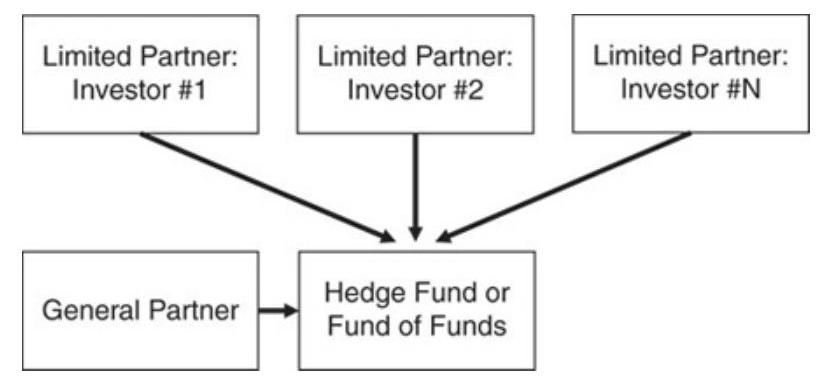
\includegraphics[max width=\textwidth]{2024_04_10_4befcf0ec10e9bee26edg-2}
\end{center}

\section*{Structure of a Limited Partnership Investment Vehicle}
Note, however, that the exhibit above is a simplification of the typical limited partnership structure as used in practice. The general partners likely formed an LLC (let's call it the "parent LLC") that in turn formed an LLC to serve as the general partner and another LLC to serve as the investment adviser to the partnership. The\\
personnel involved in three LLCs may be overlapping or even identical, with the primary functions being preserving liability and providing clarity with regard to control.

\section*{Bankruptcy-Remote Entities}
The discussions of limited liability in the previous sections focused on protecting the owners of an entity from unlimited losses generated by the entity. This section discusses protecting asset owners from the potential losses and delays from bankruptcy proceedings. A bankruptcy-remote entity is often structured as a special purpose vehicle or entity. A special purpose vehicle (SPV) or special purpose entity (SPE) is a legal entity such as an LLC that serves a specific function (such as holding assets), often with the goal of being bankruptcy remote. A bankruptcy-remote entity is designed to provide protection from involvement in potential bankruptcy proceedings of the entities placing assets in the vehicle, and is discussed further in the CDO Structuring of Credit Risk session on collateralized debt obligations. Understanding SPVs/SPEs can help clarify complex diagrams of organizational relationships.

\section*{Entities Facilitating Investor Taxation Differences}
Another organizational complexity can be master-feeder funds, which are designed to provide efficient access to investors who are subject to different taxation but wish to invest in the same portfolio. Investors with U.S. tax liability would invest in onshore funds, which are structured as U.S.-domiciled vehicles subject to U.S. regulation and tax laws. Tax-exempt investors or those who owe taxes in another country may invest offshore, such as in funds domiciled in the Cayman Islands or other offshore domiciles. Offshore jurisdictions typically do not charge taxes on investment income in the country of the fund's domicile, but trust that investors will pay taxes on the investment income in their home country. Offshore vehicles should not be used to evade taxes, as they are designed to be efficient tax-neutral vehicles that investments appropriate for asset owners, with a wide array of home countries and tax regimes. Investors in offshore funds continue to be subject to taxation in their home jurisdiction.

A fund manager may manage assets, as illustrated in the exhibit, Typical Master/Feeder Hedge Fund Structure. The master trust is the legal structure (typically offshore) used to invest the assets of both onshore investors and offshore investors in a consistent if not identical manner, so that both types of investors can share the manager's skills. Investors access the master trust through feeder funds. A feeder fund is a legal structure through which investors with common preferences with regard to taxation can have efficient access to the investment performance of the master trust. In the simplified case of two types of investors (onshore and offshore), the investors use separate feeder funds to access the master trust. Investors in both of these feeder funds benefit from the separation of funds because tax consequences flow appropriately to each investor. Together, the master trust and feeder funds are referred to as a master-feeder structure.

\begin{center}
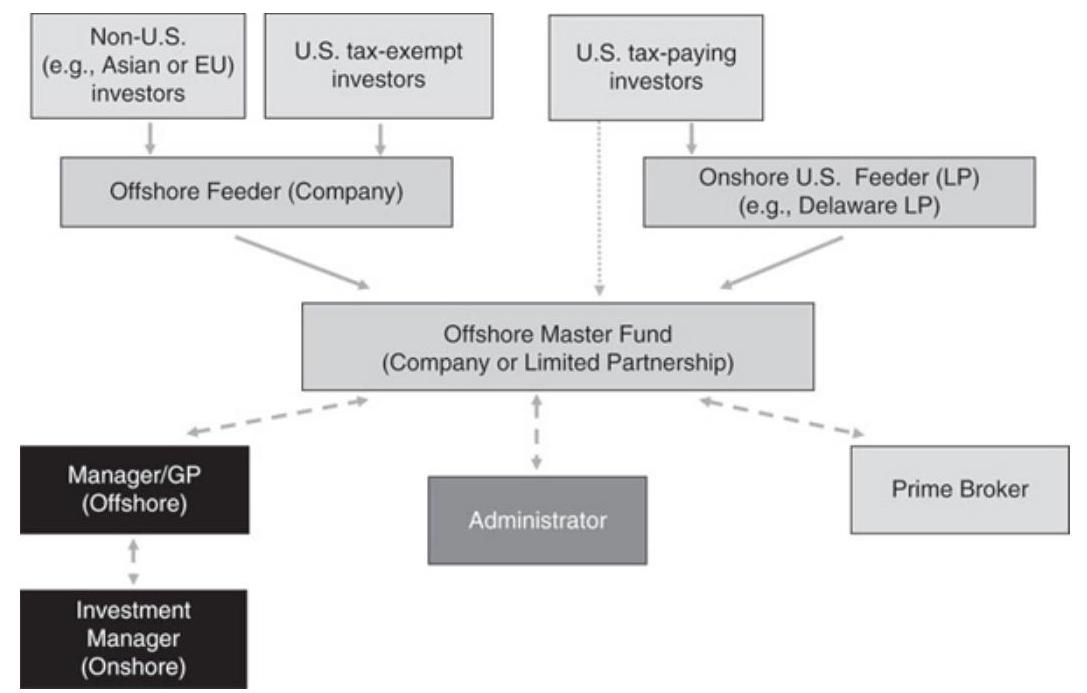
\includegraphics[max width=\textwidth]{2024_04_10_4befcf0ec10e9bee26edg-3}
\end{center}

Typical Master/Feeder Hedge Fund Structure

Source: Slide 19, "Typical Master/Feeder Hedge Fund Structure," from AIMA PowerPoint presentation "Introduction to Hedge Funds and the Alternative Investment Management Industry," November 7, 2017.

The purpose of the master trust is tax neutrality, not evasion. In Bermuda, for example, master trust funds pay only a corporate licensing fee, not corporate income tax. This ensures that there are no tax consequences to the fund investors at the master trust level. Instead, the tax consequences for the investors occur at their country of domicile based on the relevant feeder fund. Investors in the onshore, or U.S.-based, feeder fund are subject to the U.S. Internal Revenue Code, whereas investors in the offshore feeder fund are subject to the tax codes of their respective domiciles.


\end{document}